\section{Finite excitation}

For the three values of $Q$ we now consider a situation with a finite excitation time such that $F(t) = F_0 \cos(\omega t)$ for $0 < t < T$ and $F(t) = 0$ for $t \geq T$. We can solve $x(t)$ analytically, using the result for a driving force of $F(t) = F_0 \cos(\omega t)$ for $t > 0$. Using this, we can find $x(T)$ and $\dot{x}(T)$. Subsequently, We can use this as the initial conditions in the same function $x(t)$, however with $F_0 = 0$. We also need to shift the function $t=T$ to future.

\begin{align*}
	x(t)(t) = \begin{cases}
		x_1(t) & , \; 0 < t < T \\
		x_2(t-T) & , \; t \geq T \\
		\end{cases}
\end{align*}

With:

\begin{align*}
	x_1(t) = c_1 y_1(t) + c_2 y_2(t) + \frac{F_0 Q}{\omega^2 m}\sin(\omega t) \\
	x_2(t) = d_1 y_1(t) + d_2 y_2(t)
\end{align*}

$c_1$, $c_2$, $y_1$ and $y_2$ are defined as in the previous section and for $d_1$ and $d_2$:

\begin{align*}
	d_1 = \frac{1}{r_2-r_1} \left( -\dot{x}_1(T) + x_1(T) r_2 \right) \\
	d_2 = \frac{1}{r_2-r_1} \left( \dot{x}_1(T)  - x_1(T) r_1 \right) \\
\end{align*}

We can plot graphs for the values $\omega T = 0.1$, $\omega T = 1$ and $\omega T = 10$ for the three discussed values of $Q$. A scaled version of $F(t)$ is also plotted in the same axes in order to study the system with respect to the driving force:

\begin{figure}[h!]
	\centering
	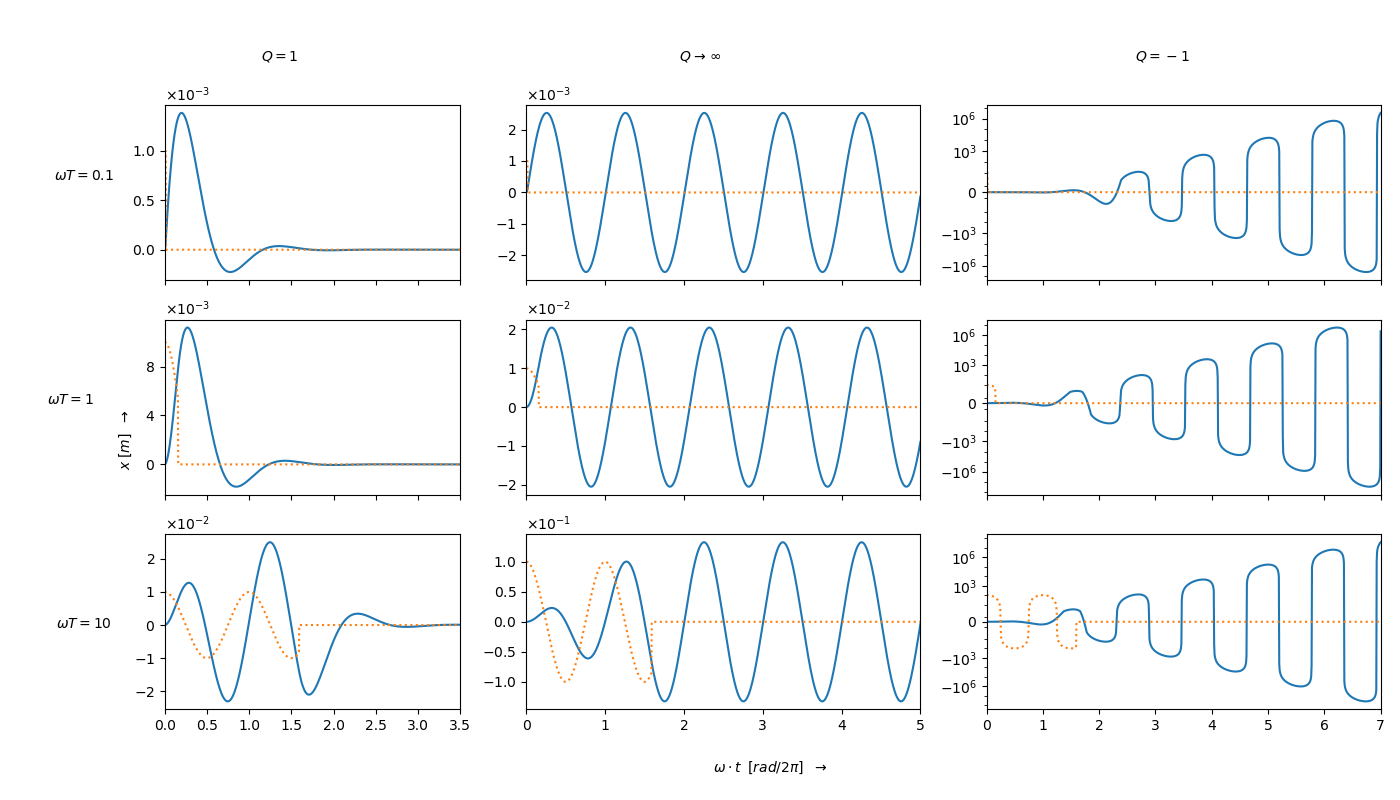
\includegraphics[width=0.8\textwidth]{figures/graph_q2.png}
	\caption{Graphs of $x(t)$ and $F(t)$  as function of $t$ for different values of $Q$ and $T$. The solid blue lines correspond with $x(t)$ and the orange dashed lines correspond to a scaled version of $F(t)$.}
	\label{fig_q1}
\end{figure}

We can make a number of observations from the graphs. Considering $Q = 1$, we find that , when there is no driving force, $x(t)$ will converge to zero. This is logical, since for $t>T$, there is only energy dissipation in the system by the friction. We also see that the graphs for $\omega T = 0.1$ and $\omega T =1$, the graphs are practically of identical shape, only differing by the amplitude and a slight time shift. The graph for $\omega T = 10$ shows that the shape of $x(t)$ is very different when $T$ is in a different phase of the oscillation.
For $Q \rightarrow \infty$ we find that for $t=T$, the oscillator will reach a steady state. This is logical since there is no energy dissipation or work done on the system. Therefore, the total energy in the system will remain constant. The amplitude of the steady state is the amplitude that corresponds with the energy in the system at $t=T$. We also see that the peaks of the three graphs are relatively close to each other. We can conclude from the graphs that the value of $T$ does not affect the shape of $x(t)$ and hardly affects the phase for an oscillator without friction. The amplitude is related to the excitation time.
For $Q=-1$ we see that the three graphs are very similar of shape, phase. Considering the logarithmic scale on the graphs, relative amplitude between $\omega T = 10$ and $\omega T = 0.1$ is more than a factor ten. The graphs do show some differences in shape in the long term. However, after about 2 oscillations, these differences become indiscernible. What's more is the amplification of the amplitude which seems equally for the three graphs and similar to the case with infinite excitation time in the previous section. It seems as for this system with 'inverse' friction. therefore, it seems as if the excitation time does not make a considerable difference to the system in the long term.